%  http://latex-beamer.sourceforge.net/

%\documentclass[landscape]{foils}

%\documentclass{beamer}
%\documentclass[handout]{beamer}     % TO PRINT PRESENTATION HANDOUT
\documentclass[xcolor=dvipsnames]{beamer}  % ALLOWS CHANGE IN COLOR

\usepackage{color}

\usepackage{pifont} %para tener la ballot cross \ding{55}

\usepackage{beamerthemesplit}
\usepackage{url}
\usepackage{ae} % or {zefonts}
\usepackage[T1]{fontenc}
\usepackage[ansinew]{inputenc}
\usepackage[spanish,es-nodecimaldot]{babel}

\usepackage{graphicx}
%\graphicspath{"c:/data"}
\usepackage{color}
%\usepackage[colorlinks]{hyperref}
\usepackage{tikz} % Easier syntax to draw pgf files (invokes pgf automatically)
\usetikzlibrary{arrows,shapes.geometric}
%\usepackage{pgfmath} % new version of Tikz loads package automatically

\usepackage{tabulary} %calcula autom�ticamente ancho de columnas con texto muy largo
%% usar LRJC para c�lculo autom�tico, lrjc para ancho de columna normal
\setlength\tymin{10pt}       %% estos permiten cambiar conducta, ver p. 254 LaTeX companion
\setlength\tymax{\maxdimen}

%\usecolortheme{crane}     %Color yellow
%\usetheme{Warsaw}
\usecolortheme[named=Gray]{structure}

\useoutertheme[footline=empty]{}  % PUTS COLORED LINE AT FOOT WITH TITLE, AUTHOR, PAGE, etc
%\usetheme{Berkeley}
\usetheme[height=7mm]{Rochester}
\setbeamertemplate{items}[ball]   % ITEMS IN 3D BALLS (alt CIRCLES)
\setbeamertemplate{navigation symbols}{}  % DROPS NAVIGATION ICONS
\setbeamertemplate{blocks}[rounded][shadow=true]

\usepackage{multirow} %allows multiple rows in tables

%\setbeamertemplate{footline} {
%    \begin{beamercolorbox}{section in head/foot}
%    \insertsectionnavigationhorizontal{\paperwidth}{}{plus1filll
%    \insertframenumber}
%    \end{beamercolorbox}
%}

%\setbeamertemplate{navigation symbols}{\insertslidenavigationsymbol, \insertdocnavigationsymbol} 
\setbeamertemplate{footline} {
    \begin{beamercolorbox}{section in head/foot}
    \insertsectionnavigationhorizontal{\paperwidth}{}{plus1filll
%    \insertslidenavigationsymbol \insertdocnavigationsymbol \insertframenumber}
    \insertframenumber}
    \end{beamercolorbox}
}

\setbeamercovered{transparent}
\setbeamertemplate{caption}{\insertcaption}

%\tikzstyle{nodo} = [circle, draw=black, fill=white, text=black]
%\tikzstyle{end} = [circle, minimum width=3pt,fill, inner sep=0pt]

\title[PAN y reformas]{El PAN ante \\ las reformas pendientes}
%\subtitle{}
\author[Magar]{Eric Magar}
\institute[ITAM]{ITAM--Ciencia Pol�tica}
\date[30nov12]{20 de noviembre 2013}

\AtBeginSection[] % Do nothing for \section*
{
  \begin{frame}<beamer>
  \frametitle{Contenido}
  \tableofcontents[currentsection]
  \end{frame}
}

\begin{document}

%%%%%%%%%%%%%%%%%%%%%%%%%%%%%%%%%%%%%%%%%%%%%%%%%%%%%%%%%%%%%%%%%%%%%%%%%%%%%%%%%%%%%%%%%%%%

\frame[plain]{\titlepage}

%%%%%%%%%%%%%%%%%%%%%%%%%%%%%%%%%%%%%%%%%%%%%%%%%%%%%%%%%%%%%%%%%%%%%%%%%%%%%%%%%%%%%%%%%%%%
\frame {                      % SLIDE

    \frametitle{Dos grandes temas}

\begin{enumerate}

\item La reforma energ�tica

  \begin{itemize}
 
    \item �Fin del pacto?
    \item Condicionarla
    \item La dimensi�n temporal

  \end{itemize}
    
\item La reforma pol�tica

  \begin{itemize}

    \item Reelecci�n legislativa
    \item Tama�o del congreso
    \item Redistritaci�n

  \end{itemize}

\end{enumerate}

%  \begin{columns}[c]

%  \column{.45\textwidth}

% \emph{Arrastre presidencial} = ganador de la contienda presidencial ``jala'' a sus copartidarios hacia la victoria en la pista congresional

%  \column{.55\textwidth}

% % \includegraphics[width=6cm]{bush2002.pdf}

%  \end{columns}


}

%%%%%%%%%%%%%%%%%%%%%%%%%%%%%%%%%%%%%%%%%%%%%%%%%%%%%%%%%%%%%%%%%%%%%%%%%%%%%%%%%%%%%%%%%%%%
\frame {                      % SLIDE

    \frametitle{Quitar diputados afecta al PAN}

Por el tama�o del pa�s, la c�mara de diputados est� en el promedio mundial

\bigskip

\begin{center}

Victorias uninominales 

\begin{tabular}{rrrrr}
     & PAN & PRI & PRD & otros \\ \hline
2006 & 134 &  65 & 101 &    0 \\
2009 &  71 & 187 &  39 &    3 \\
2012 &  52 & 174 &  71 &    3 \\
\end{tabular}
\end{center}

}
%%%%%%%%%%%%%%%%%%%%%%%%%%%%%%%%%%%%%%%%%%%%%%%%%%%%%%%%%%%%%%%%%%%%%%%%%%%%%%%%%%%%%%%%%%%%
\frame {                      % SLIDE

    \frametitle{La relaci�n votos--esca�os}

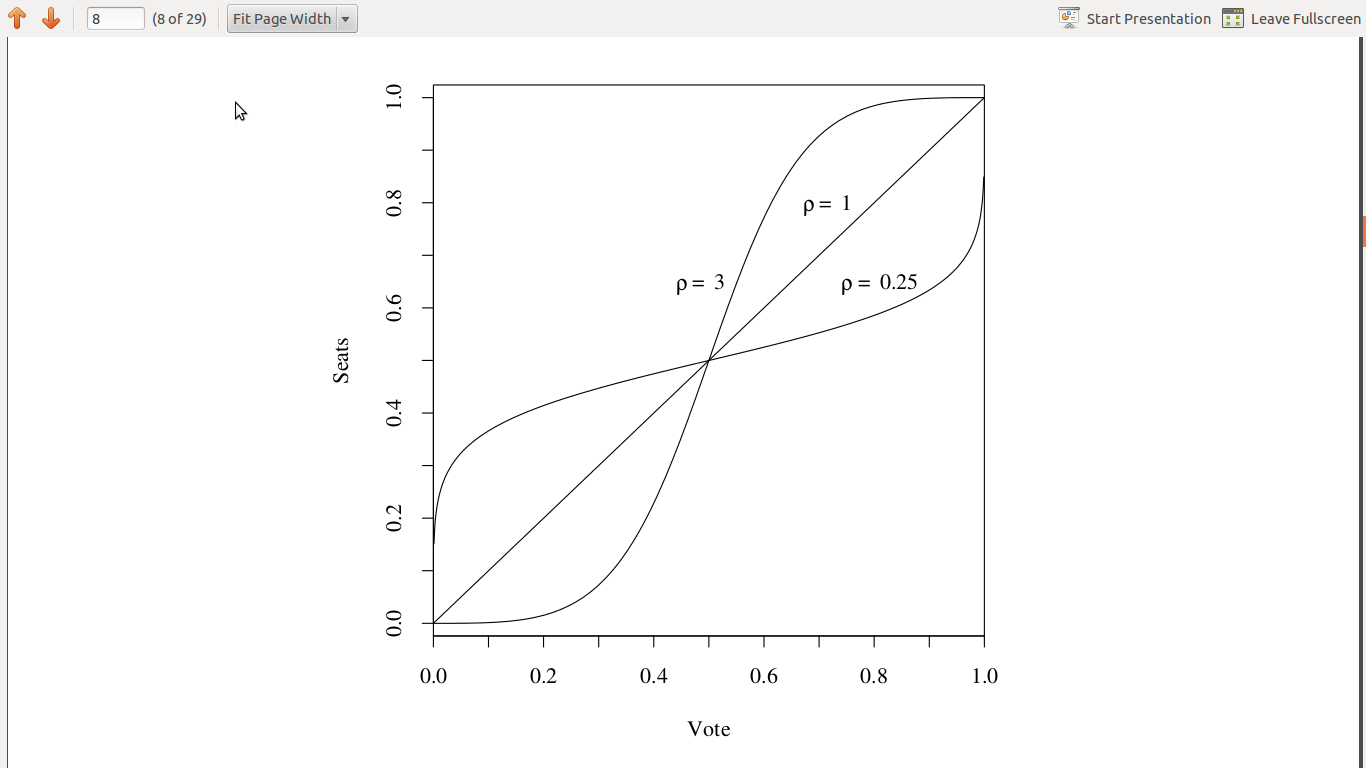
\includegraphics[width=12cm]{../graphs/rho.png}

}

%%%%%%%%%%%%%%%%%%%%%%%%%%%%%%%%%%%%%%%%%%%%%%%%%%%%%%%%%%%%%%%%%%%%%%%%%%%%%%%%%%%%%%%%%%%%
\frame {                      % SLIDE

    \frametitle{La relaci�n votos--esca�os}

\begin{center}
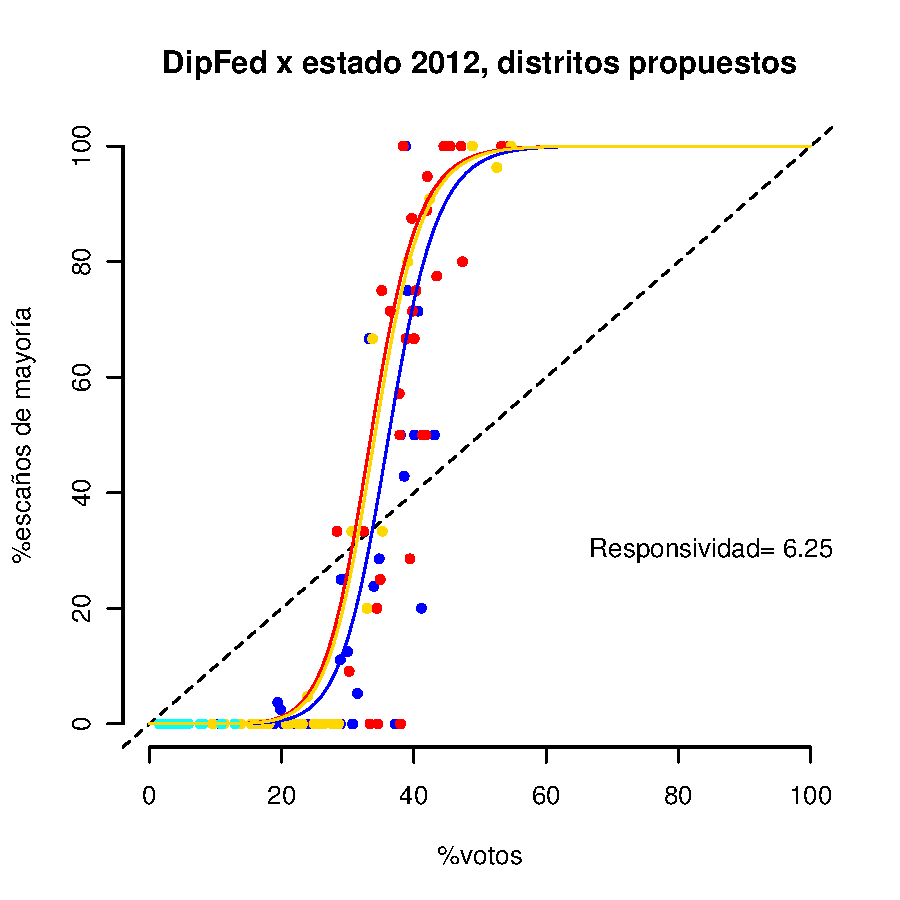
\includegraphics[width=8cm]{../graphs/biasResp2012s3.pdf}
\end{center}
}

%%%%%%%%%%%%%%%%%%%%%%%%%%%%%%%%%%%%%%%%%%%%%%%%%%%%%%%%%%%%%%%%%%%%%%%%%%%%%%%%%%%%%%%%%%%%
\frame {                      % SLIDE

    \frametitle{La relaci�n votos--esca�os}

\begin{center}
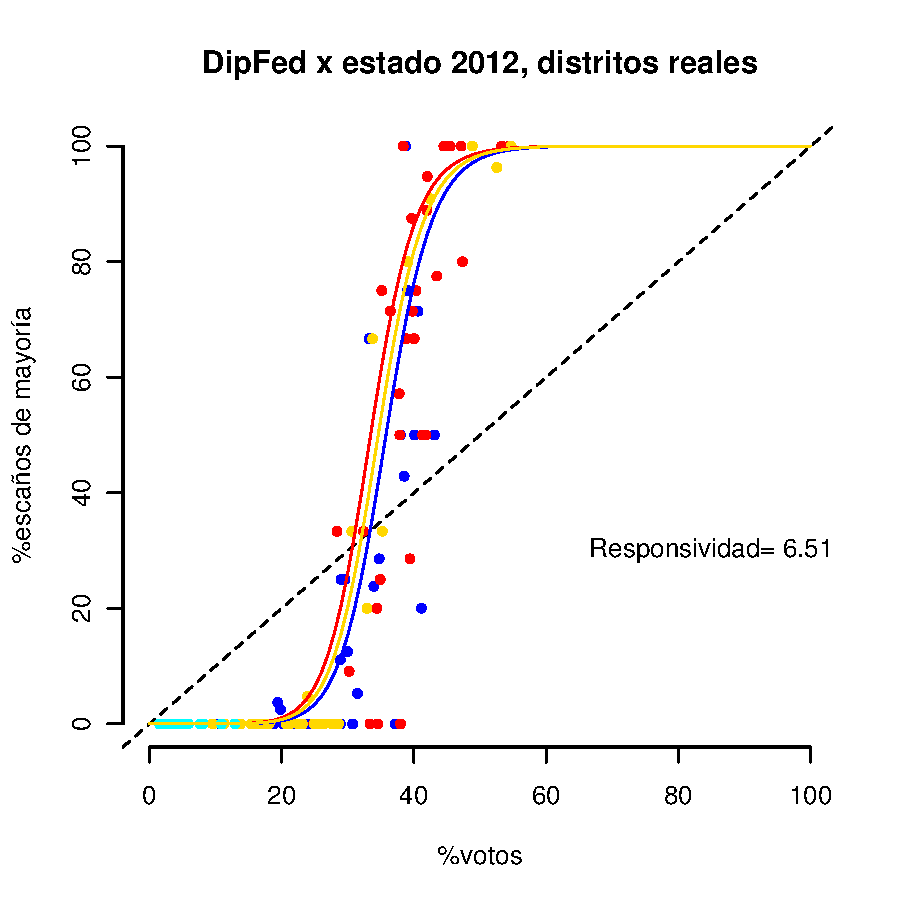
\includegraphics[width=8cm]{../graphs/biasResp2012s0.pdf}
\end{center}
}

%%%%%%%%%%%%%%%%%%%%%%%%%%%%%%%%%%%%%%%%%%%%%%%%%%%%%%%%%%%%%%%%%%%%%%%%%%%%%%%%%%%%%%%%%%%%
\frame {                      % SLIDE

    \frametitle{La relaci�n votos--esca�os}

\begin{center}
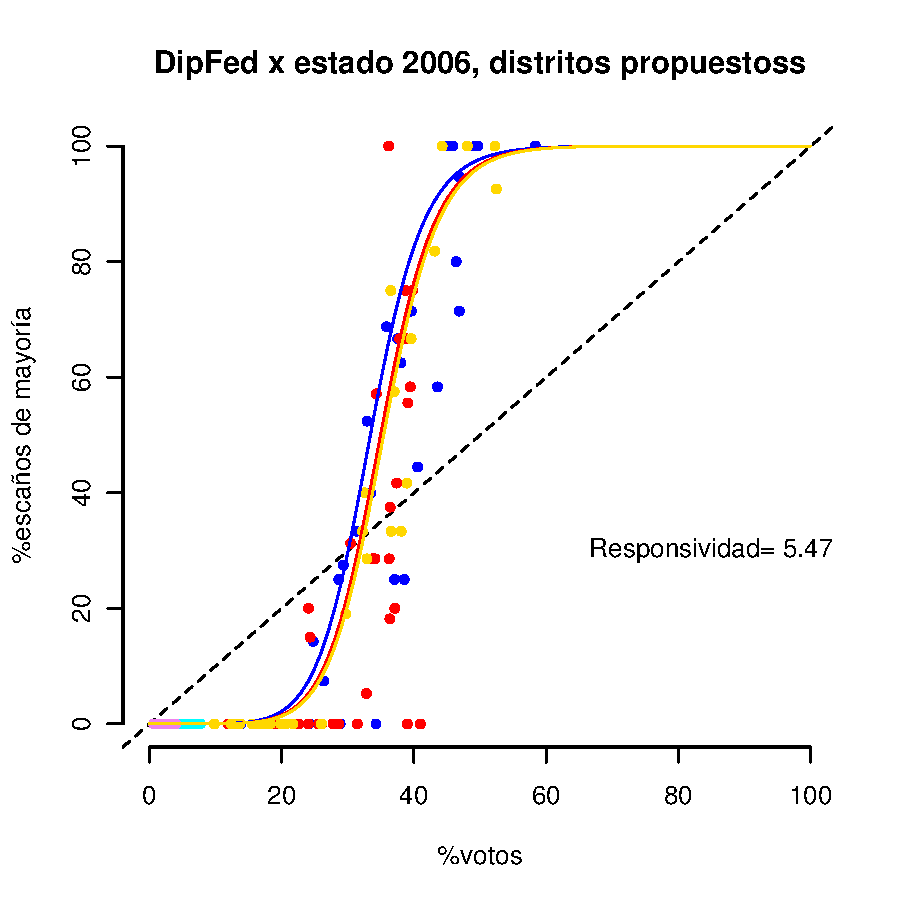
\includegraphics[width=8cm]{../graphs/biasResp2006s3.pdf}
\end{center}
}

%%%%%%%%%%%%%%%%%%%%%%%%%%%%%%%%%%%%%%%%%%%%%%%%%%%%%%%%%%%%%%%%%%%%%%%%%%%%%%%%%%%%%%%%%%%%
\frame {                      % SLIDE

    \frametitle{La relaci�n votos--esca�os}

\begin{center}
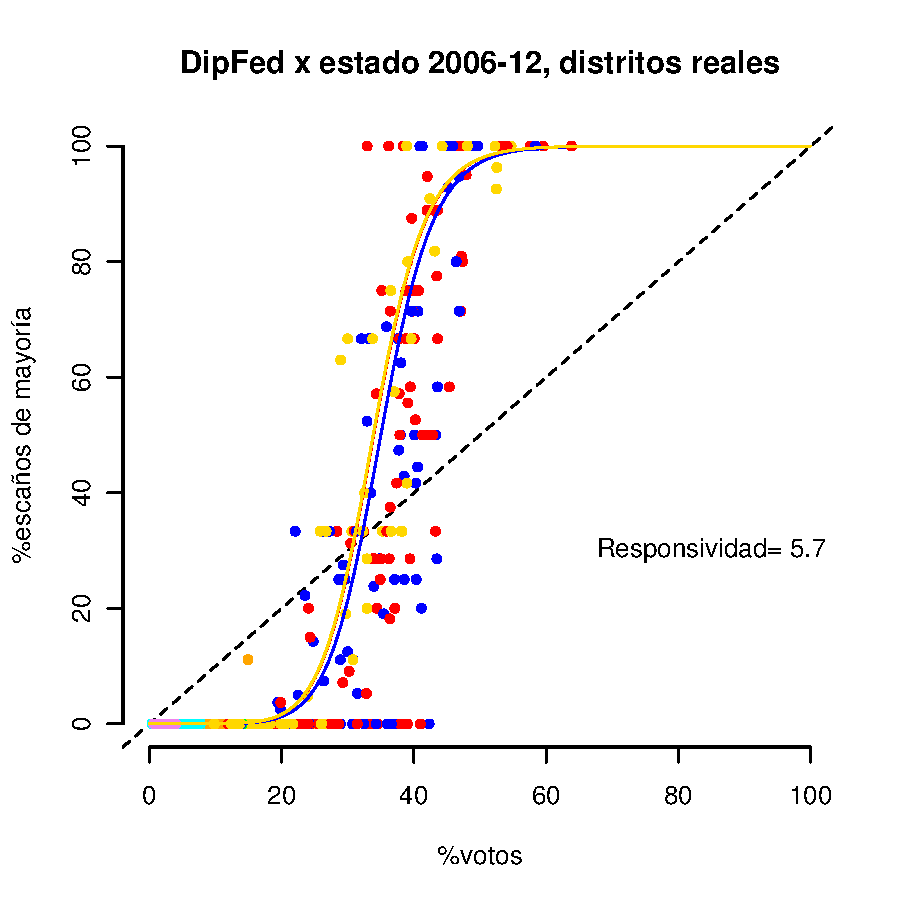
\includegraphics[width=8cm]{../graphs/biasResp2006-12s0.pdf}
\end{center}
}

%%%%%%%%%%%%%%%%%%%%%%%%%%%%%%%%%%%%%%%%%%%%%%%%%%%%%%%%%%%%%%%%%%%%%%%%%%%%%%%%%%%%%%%%%%%%
\frame {                      % SLIDE

    \frametitle{La relaci�n votos--esca�os}

\begin{center}
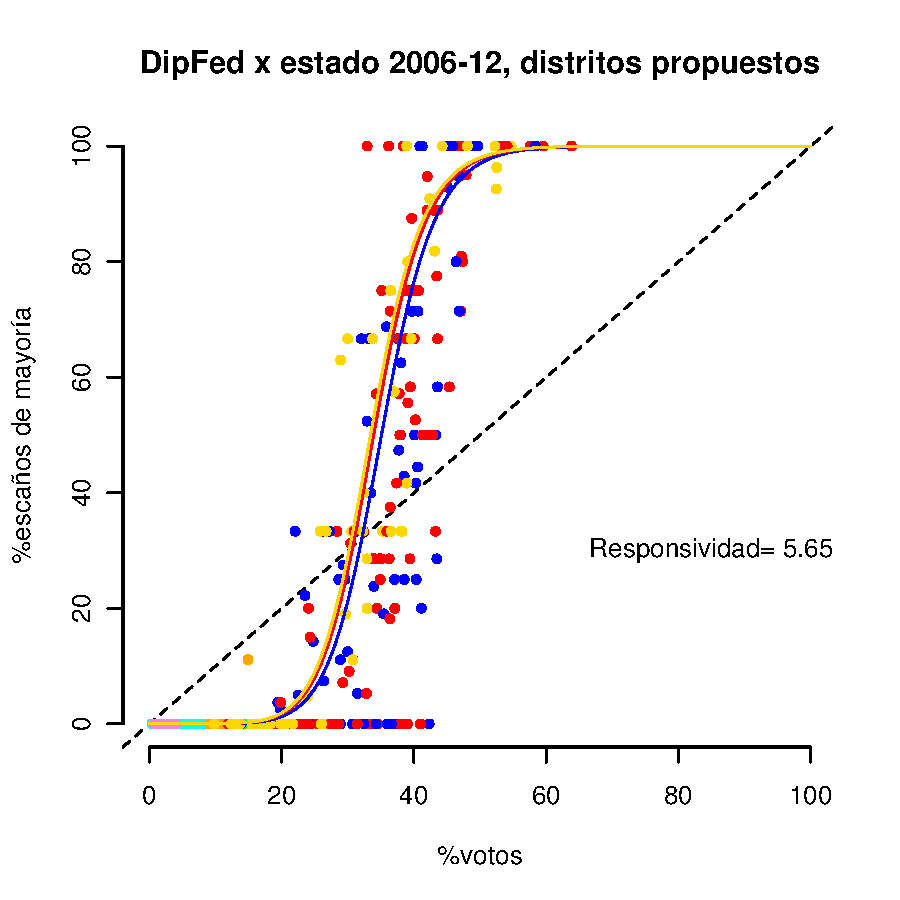
\includegraphics[width=8cm]{../graphs/biasResp2006-12s3.pdf}
\end{center}
}

%%%%%%%%%%%%%%%%%%%%%%%%%%%%%%%%%%%%%%%%%%%%%%%%%%%%%%%%%%%%%%%%%%%%%%%%%%%%%%%%%%%%%%%%%%%%
\frame {                      % SLIDE

    \frametitle{La relaci�n votos--esca�os}

\begin{center}
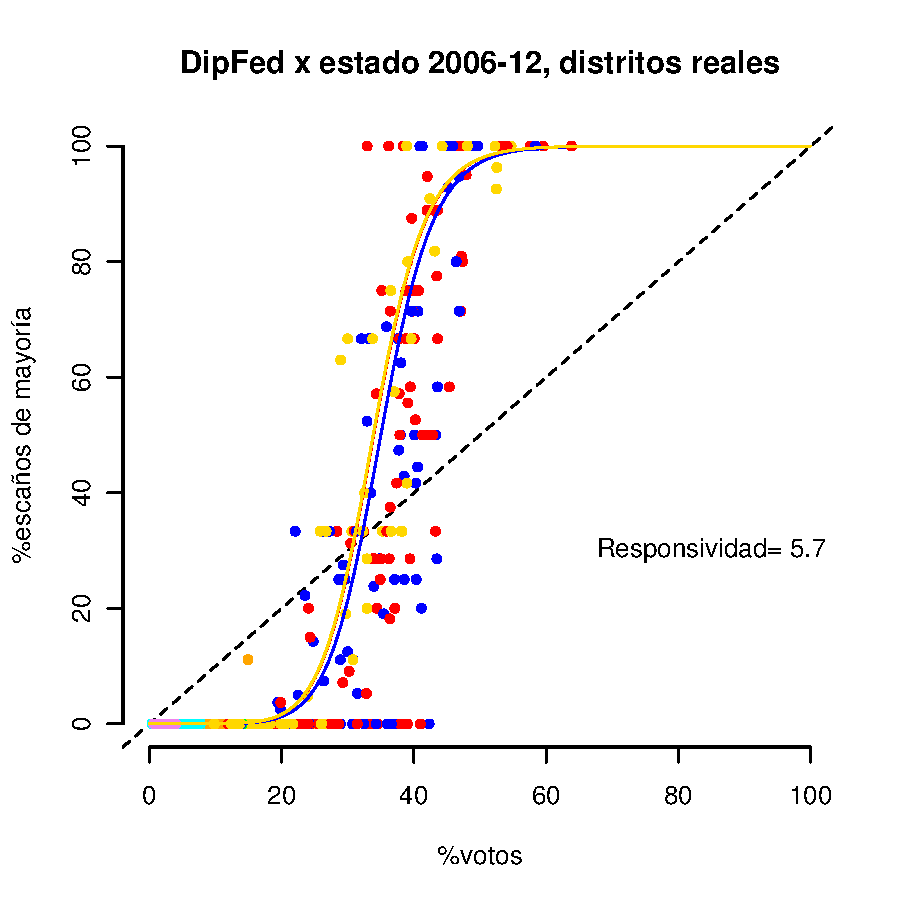
\includegraphics[width=8cm]{../graphs/biasResp2006-12s0.pdf}
\end{center}
}

%%%%%%%%%%%%%%%%%%%%%%%%%%%%%%%%%%%%%%%%%%%%%%%%%%%%%%%%%%%%%%%%%%%%%%%%%%%%%%%%%%%%%%%%%%%%
\frame {                      % SLIDE

    \frametitle{En resumen}

    \begin{itemize}
     \item Energ�tica: Pe�a tiene el voto del PAN cautivo
     \item Atrasar es la mejor carta
     \item La reelecci�n legislativa ser�a excelente logro
     \item No redistritar afecta al PAN
    \end{itemize}

\bigskip
\pause

    \begin{center}
      \textbf{�Gracias!}
    \end{center}
}

\end{document}

